\section{Introduction}
There are three main types of communicating wirelessly underwater -
acoustic, RF and optical. Acoustic transmissions are characterized by
long range but low data rates. RF transmissions are characterized by
high throughput but only at very short distances. Optical transmissions
sit halfway between these, allowing high throughput at medium ranges,
but at the expense of being affected by the environment of the wireless
channel.

\begin{figure}[H]
  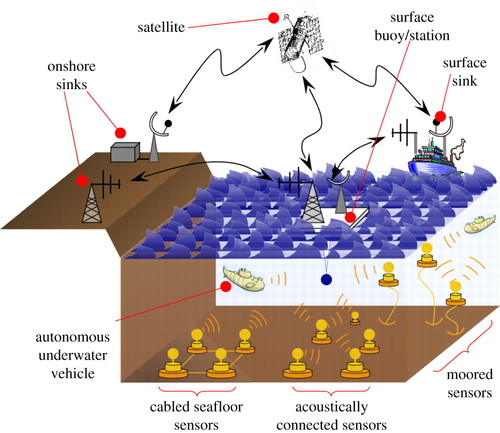
\includegraphics[width=0.8\textwidth]{underwater_network_topologies.jpg}
  \caption{Generic Underwater Network Topologies}
  \label{fig:underwater_network_topologies}
\end{figure}